\documentclass{article}

\usepackage{../../preamble}

\title{PGM: Homework 1}
\author{Raphael Reme}

\begin{document}
\maketitle

\section{Noisy Ising}
Consider a simple version of the Ising model:
\begin{equation*}
    p(x) = \frac{1}{Z_{\alpha, \beta}} \exp\left\{ \alpha \sum_{i=1}^nx_i + \beta \sum_{(i,j) \in E} \mathds{1}(x_i = x_j)\right\}
\end{equation*}
where the $x_i$ are either $0$ or $1$. Recall that $(i, j) \in E$ means that there is an edge between nodes $i$ and $j$, and
that $\mathds{1}(x_i = x_j)$ is one if $x_i$ and $x_j$ have the same ”colour”, zero otherwise.

We do not observe $x$ directly. Instead, we observe independent variables $y_i$ which, conditional on $x_i = l$
are distributed according to a Gaussian distribution $\mathcal{N}(\mu_l, 1)$. This type of model is often used for grayscale
images, like this one:

\begin{figure}[h!]
    \centering
    
\includegraphics[width=0.5\linewidth]{spiral}
    \label{fig:spiral}
\end{figure}

(You can use another, more interesting gray-scale image, but don’t forget to add some level of noise!)
We first treat the parameters $\alpha, \beta, \mu_0, \mu_1$ as fixed.

\paragraph*{1-} Explain the trick we may use to adapt belief propagation to the problem of computing the distribution
of a given $x_i$, conditional on all the $y_i$’s. Is this algorithm exact? Explain. Implement the algorithm.
\paragraph*{Answer} First let's express the join probability:
\begin{equation*}
    \begin{aligned}
        p(x, y) & = p(x)p(y|x)                                      &  & \text{(Bayes formula)}                                                                      \\
                & = p(x)\prod_{i=1}^np(y_i|x_i)                     &  & \text{($y_i$ is independent of $x_j$ and $y_i|x_i$ is independent of $y_j$ for $j \neq i$)} \\
                & = p(x)\prod_{i=1}^n\mathcal{N}(y_i; \mu_{x_i}, 1)                                                                                                  \\
    \end{aligned}
\end{equation*}

Finally we have
\begin{equation*}
    \begin{aligned}
        p(x, y) & = \frac{1}{Z_{\alpha, \beta}} \exp\left\{ \alpha \sum_{i=1}^nx_i + \beta \sum_{(i,j) \in E} \mathds{1}(x_i = x_j)\right\}\prod_{i=1}^n\mathcal{N}(y_i; \mu_{x_i}, 1) \\
                & \propto \prod_{i=1}^ne^{\alpha x_i} \prod_{(i, j) \in E}e^{\beta \mathds{1}(x_i = x_j)}\prod_{i=1}^n\mathcal{N}(y_i; \mu_{x_i}, 1)                                   \\
                & \propto \prod_{i=1}^n \psi_1(x_i) \prod_{(i, j) \in E} \psi_2(x_i, x_j) \prod_{i=1}^n \psi_3(x_i, y_i)                                                               \\
    \end{aligned}
\end{equation*}

With $\psi_1(x_i) = e^{\alpha x_i}, \psi_2(x_i, x_j) = e^{\beta \mathds{1}(x_i = x_j)}, \psi_3(x_i, y_i) = e^{-\frac{1}{2}(y_i-\mu_{x_i})^2}$.

It defines the a classical graph for images where we have a node for each pixel ($x_i$) with edges with its
4 neighbours. And one node for each pixel ($y_i$) with an unique edge to the corresponding $x_i$. And we will observed the $y_i$ and try to deduce
the law of $x_i$ given this observation.

Let's try to express $p(x|y)$:

\begin{equation*}
    \begin{aligned}
        p(x| y) & \propto p(x, y)                                                                                        \\
                & \propto \prod_{i=1}^n \psi_1(x_i) \prod_{(i, j) \in E} \psi_2(x_i, x_j) \prod_{i=1}^n \psi_3(x_i, y_i) \\
                & \propto \prod_{i=1}^n \psi_1(x_i) \psi_3(x_i, y_i) \prod_{(i, j) \in E} \psi_2(x_i, x_j)               \\
                & \propto \prod_{i=1}^n \psi_4(x_i) \prod_{(i, j) \in E} \psi_2(x_i, x_j)                                \\
    \end{aligned}
\end{equation*}

With $\psi_4(x_i) = \psi_1(x_i)\psi_3(x_i, y_i)$ ($y_i$ are as constants here.) This leads to a simpler graph where the $y_i$ nodes have vanished.

But even with this simplification we end up with a cycling graph. Therefore the Belief Propagation algorithm does not work. Nonetheless there are at least
two solutions for this. First, we could try to group nodes together (Line by line or try to be smarter). The point is to reduce our cycling graph to a tree
and then use the Belief Propagation algorithm. This is the Junction Tree method. It is exact, but very costly with an image of this size. (As each
"super" node has a lot of possible values)

I would rather use the second possibility: the Loopy Belief Propagation method, which consists in randomly initalize all the messages and update them until
they converge.  It's not an exact solution but it's often a good one and it's much cheaper to execute.

Let's define the messages for a pixel $k$ from one of it's neighbor $j$:

\begin{equation*}
    \mu_{j \rightarrow k}(x_k) = \sum_{x_j} \psi_2(x_j, x_k) \psi_4(x_j) \prod_{i\in\text{ne}(j)\setminus\{k\}}\mu_{i \rightarrow j}(x_j)
\end{equation*}

Note than in our graph, messages can pass in only 4 directions at each pixel: Up, Down, Right, Left. (At each pixel there are at most four
incoming messages.)

Once we have computed these messages with the Loopy Belief Propagation method, we can compute $p(x_k|y)$:
\begin{equation*}
    p(x_k| y) \propto \psi_4(x_k) \prod_{j \in \text{ne}(k)} \mu_{j \rightarrow k}(x_k)
\end{equation*}

\paragraph*{Practical implementation}
I implemented the Loopy Belief Propagation for this model. I choose $\alpha = 0$ and good values of
$\beta$ for this image seem to be greater than $0.6$.

For visual testing purpose I tried to approximate $x^\star = \text{argmax}_x p(x|y)$ with $(x_i^\star)_i$
where each \\$x_i^\star = \text{argmax}_{x_i} p(x_i|y)$. If the algorithm works well, this image "should" approximate
the initial distribution and thus should be denoised.

To reproduce results the code can be run with:
\begin{lstlisting}{bash}
    $ python belief.py path/to/image.png -N 20 --mu-0 0.1 --mu-1 0.9
\end{lstlisting}

One can see that it denoises the image and thus it seems that the algorithm works. (Note that we stop the algorithm after N steps
because the convergence is very slow and the results are quite good and does not changed a lot after N > 5)

\begin{figure}[h!]
    \centering
    \begin{subfigure}[b]{0.3\linewidth}
        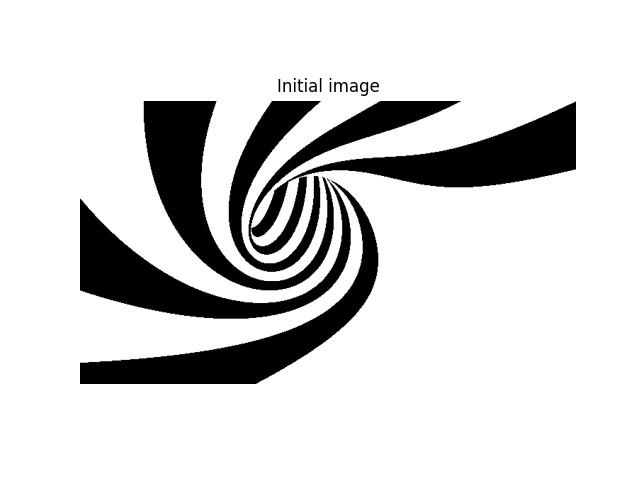
\includegraphics[width=\linewidth]{initial.png}
    \end{subfigure}
    \begin{subfigure}[b]{0.3\linewidth}
        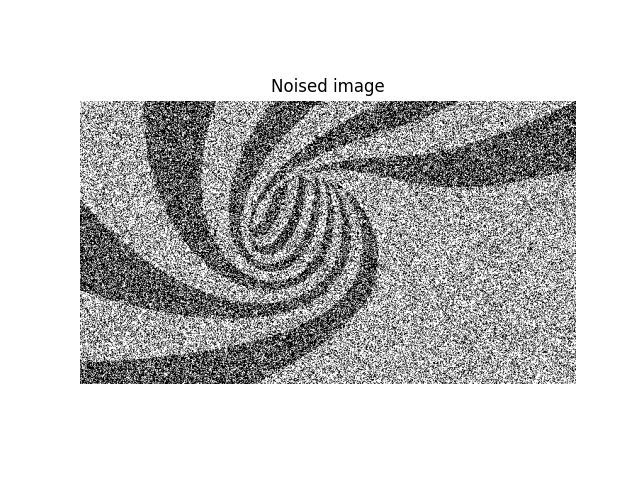
\includegraphics[width=\linewidth]{noisy.png}
    \end{subfigure}
    \begin{subfigure}[b]{0.3\linewidth}
        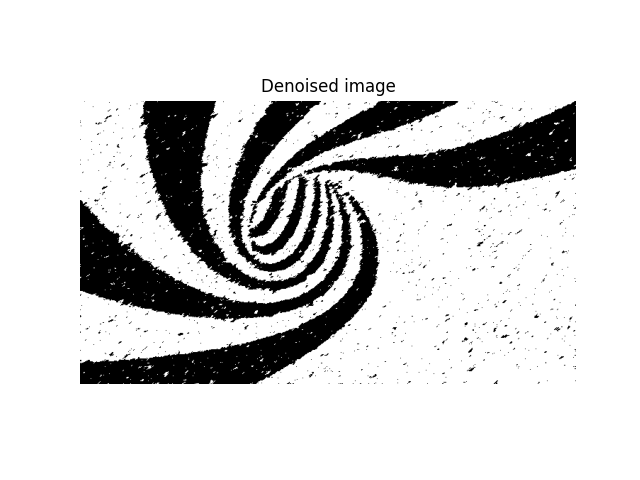
\includegraphics[width=\linewidth]{denoised.png}
    \end{subfigure}
    \caption{Denoising image using the Loopy Belief Propagation (Sum-Product)}
    \label{fig:LBP}
\end{figure}

\paragraph*{2-} Explain how you may instead use MCMC to sample from the same conditional distribution. Compute
any distribution you need to sample from, and explain why these distributions are easy to sample from.
Implement the corresponding MCMC algorithm.

\paragraph*{Answer}


\end{document}